% -*- coding: utf-8 -*-

\documentclass[b5paper,papersize,tombow,11pt]{jsbook}

\usepackage{amsmath,ascmac}
\usepackage{graphicx}
\usepackage{lettrine}
\usepackage{fancyhdr}
\usepackage{fancybox}
\usepackage{listings}
% Palatino
\usepackage{palatino}

%% Page Layout
% B5: 182mm x 257mm
\setlength{\voffset}{0mm}
\setlength{\topmargin}{-15mm}
\setlength{\textheight}{34\Cvs}
\setlength{\textwidth}{\fullwidth}
\setlength{\footskip}{10mm}

% set margin for openleft
% \setlength{\oddsidemargin}{-\oddsidemargin}
% \setlength{\evensidemargin}{-\oddsidemargin}


\pagestyle{fancy}

\fancyhead{}
% \fancyhead[RO,RE]{\rightmark}
% \fancyhead[LE,LO]{\leftmark}
\fancyhead[RO]{\rightmark}
\fancyhead[LE]{\leftmark}
\cfoot{\bfseries -- \thepage \ --} % page number at the center bottom
\renewcommand{\headrule}{
\vskip -1.5mm
\hskip-0.03\textwidth
\includegraphics[width=1.06\textwidth,height=3.78mm]{hayamiz/images/hrule.eps}
\vskip -2.28mm
}

% jsbook.cls use 'plainhead' style for the first page of each chapter
\fancypagestyle{plainhead}{
\fancyhf{}
\cfoot{\bfseries -- \thepage \ --}
\renewcommand{\headrulewidth}{0.0pt}
\renewcommand{\headrule}{}
}

% jsbook.cls use 'empty' style for blank
\fancypagestyle{empty}{
\fancyhf{}
\cfoot{\bfseries -- \thepage \ --}
\renewcommand{\headrulewidth}{0.0pt}
\renewcommand{\headrule}{}
}

\makeatletter
\renewcommand{\chapter}{%
  \if@openright\cleardoublepage\else\clearpage\fi
  \plainifnotempty % 元: \thispagestyle{plain}
  \global\@topnum\z@
  \if@english \@afterindentfalse \else \@afterindenttrue \fi
  \secdef\@chapter\@schapter}
\def\@chapter[#1]#2{%
  \ifnum \c@secnumdepth >\m@ne
    \if@mainmatter
      \refstepcounter{chapter}%
      \typeout{\@chapapp\thechapter\@chappos}%
      \addcontentsline{toc}{chapter}%
        {\protect\numberline
        {\if@english\thechapter\else\@chapapp\thechapter\@chappos\fi}%
        #1}%
    \else\addcontentsline{toc}{chapter}{#1}\fi
  \else
    \addcontentsline{toc}{chapter}{#1}%
  \fi
  \chaptermark{#1}%
  \addtocontents{lof}{\protect\addvspace{10\p@}}%
  \addtocontents{lot}{\protect\addvspace{10\p@}}%
  \if@twocolumn
    \@topnewpage[\@makechapterhead{#2}]%
  \else
    \@makechapterhead{#2}%
    \@afterheading
  \fi}
\def\@schapter#1{%
  \chaptermark{#1}%
  \if@twocolumn
    \@topnewpage[\@makeschapterhead{#1}]%
  \else
    \@makeschapterhead{#1}\@afterheading
  \fi}

\def\@normalchapter[#1]#2{%
  \ifnum \c@secnumdepth >\m@ne
    \if@mainmatter
      \refstepcounter{chapter}%
      \typeout{\@chapapp\thechapter\@chappos}%
      \addcontentsline{toc}{chapter}%
        {\protect\numberline
        {\if@english\thechapter\else\@chapapp\thechapter\@chappos\fi}%
        #1}%
    \else\addcontentsline{toc}{chapter}{#1}\fi
  \else
    \addcontentsline{toc}{chapter}{#1}%
  \fi
  \chaptermark{#1}%
  \addtocontents{lof}{\protect\addvspace{10\p@}}%
  \addtocontents{lot}{\protect\addvspace{10\p@}}%
  \if@twocolumn
    \@topnewpage[\@makechapterhead{#2}]%
  \else
    \@makechapterhead{#2}%
    \@afterheading
  \fi}
\def\@normalschapter#1{%
  \chaptermark{#1}%
  \if@twocolumn
    \@topnewpage[\@makeschapterhead{#1}]%
  \else
    \@makeschapterhead{#1}\@afterheading
  \fi}
\def\@makechapterhead#1{%
  {\parindent \z@ \raggedright \normalfont
    \ifnum \c@secnumdepth >\m@ne
      \if@mainmatter
        \centering\huge\headfont \@chapapp\thechapter\@chappos
        \par\nobreak
        % \vskip \Cvs % 欧文は20pt
      \fi
    \fi
    \interlinepenalty\@M
    \begin{center}
     {\LARGE \headfont #1}\par\nobreak\noindent
\hskip-0.03\textwidth
\includegraphics[width=1.06\textwidth,height=7.59mm]{hayamiz/images/chapter-title-ornament.eps}\vskip-7.59mm\vskip-0.5\Cvs
    \end{center}
    \par\nobreak
    \vskip 1.000\Cvs}} % 欧文は40pt
\def\@makeschapterhead#1{%
  {\parindent \z@ \raggedright
    \normalfont
    \interlinepenalty\@M
	\begin{center}
    {\LARGE \headfont #1}\par\nobreak\noindent
\hskip-0.03\textwidth
\includegraphics[width=1.06\textwidth,height=7.59mm]{hayamiz/images/chapter-title-ornament.eps}\vskip-7.59mm\vskip-0.5\Cvs
    \end{center}
	\par\nobreak
    \vskip 3\Cvs}} % 欧文は40pt

% section
% 後アキの調整
\renewcommand{\section}{%
  \if@slide\clearpage\fi
  \@startsection{section}{1}{\z@}%
  {\Cvs \@plus.5\Cdp \@minus.2\Cdp}% 前アキ
  {.7\Cvs \@plus.3\Cdp}% 後アキ
  {\normalfont\Large\headfont\raggedright}}

% 前・後アキの調整
\renewcommand{\subsection}{\@startsection{subsection}{2}{\z@}%
  {0.7\Cvs \@plus.5\Cdp \@minus.2\Cdp}% 前アキ
  {.25\Cvs \@plus.3\Cdp}% 後アキ
  {\normalfont\large\headfont}}


\makeatother

\renewcommand{\prechaptername}{}
\renewcommand{\postchaptername}{}

\makeatletter
\renewcommand{\thesection}{\S\,\@arabic\c@section}
\makeatother

\ifx\Cht\undefined
 \newdimen\Cht\newdimen\Cdp
 \setbox0\hbox{\char\jis2121}\Cht=\ht0\Cdp=\dp0\fi
\makeatletter
\long\def\linespace#1#2{\par\noindent
  \dimen@=\baselineskip\multiply\dimen@ #1\advance\dimen@-\baselineskip
  \advance\dimen@-\Cht\advance\dimen@\Cdp
  \setbox0\vbox{\noindent #2}\advance\dimen@\ht0\advance\dimen@-\dp0%
  \vtop to\z@{\hbox{\vrule width\z@ height\Cht depth\z@
   \raise-.5\dimen@\hbox{\box0}}\vss}%
  \dimen@=\baselineskip\multiply\dimen@ #1\advance\dimen@-\baselineskip
  \vskip\dimen@}
\makeatother

\title{The Database Times Vol. 1}
\date{2012/8/11}
\author{Hotchpotch Society}

\newcommand{\term}[2]{\noindent{\gt $\clubsuit$ #1}$\cdots$ #2}

%% Listings
\newcommand{\listingsize}{\small}
\lstset{language=SQL,
morekeywords={RETRIEVE,RANGE,OF,IS},
numbers = left,
numberstyle = {\tiny},
numbersep = 5pt,
breaklines = false,
breakindent = 40pt,
flexiblecolumns = true,
keepspaces = false,
basicstyle = \normalsize,
identifierstyle = \itshape\listingsize,
commentstyle = \fontfamily{ptm}\selectfont\listingsize,
stringstyle = \upshape\listingsize,
tabsize = 4,
escapechar = |,
}


\begin{document}

\thispagestyle{empty}

\frontmatter

% タイトルページ
\begin{center}
 
\includegraphics[width=12cm]{hayamiz/images/title.eps}
 \par\vspace*{50mm}
 \noindent Hotchpotch Society
\end{center}

% まえがきページ
% -*- coding: utf-8 -*-

\chapter*{まえがき}
\addcontentsline{toc}{chapter}{まえがき}
\thispagestyle{plainhead}

The Database Times vol.1 をお手にとっていただきありがとうございます。

本書は、データベースシステムを中心として、様々な情報技術に関する話題を読
者の皆様にお届けすることを目的としています。みなさんは「データベースシス
テム」というものにどのようなイメージをお持ちでしょうか。SQLを投げるとデー
タを返してくれる、なんだかよくわからないけれど枯れた時代遅れの技術だとい
うイメージを持っている人が多いのではないかと思います。

しかしながら、実際のデータベースシステムは古の技術を土台として、その時代
の最先端の技術が詰め込まれた非常に魅力的な技術の集大成なのです。世界中で
生み出されるデータ量がどのくらいかご存知でしょうか。2010年までに生み出さ
れたデータ量はなんと1,227ペタバイト。しかも、2020年には7,910,000ペタバイ
トになるであろうと予測されています。人類が産み出そうとしているデータ量は、
まさに爆発的な勢いで増え続けています。このデータの膨張を支える縁の下の力
持ちがデータベースシステムです。加速するデータ量の増加に伴って、データベー
スも日々進歩を続けているのです。

そんなデータベースシステムがどのようにして生まれ、そして最近ではどんな
ことが話題になっているのか、本書を通してその一端に触れ、楽しんで頂ければ
幸いです。

\begin{flushright}
 2012年 8月

Hotchpotch Society
\end{flushright}

\newpage

\subsection*{お品書き}

\noindent {\bf ■ データベースシステムの夜明け}

今の世の中、データベースシステムといえばリレーショナルデータベースシステ
ムです。そのリレーショナルデータベースシステムが、一体どのようにして生み
出されたのか、そしてどのように発展を遂げていったのか、その歴史を辿ります。

\vspace*{\Cvs}

\noindent {\bf ■ PostgreSQLカンファレンス2012 レポート}

オープンソースDBMS代表格の一つであるPostgreSQLは、最近は業務でも用いられ
ることがかなり増えてきているようです。そんな PostgreSQL の最新技術事情に
触れられる PostgreSQL カンファレンスの参加レポートをお届けします。

\vspace*{\Cvs}

\noindent {\bf ■ とある世界で一番高速なBrainfuckインタプリタ}

近年ではSAP HANAやMemSQLなどの主記憶データベースが話題となっているように、
膨大するデータ量を捌ききるための「速さ」が強く求められています。データベー
スシステムはSQLというプログラミング言語の処理系という側面も持ちあわせてお
り、言語処理系の高速な実装はデータベースシステムには必要不可欠です。言語
処理系をいかに高速にするのか、その技術について世界最速Brainfuckインタプリ
タの実装者が解説します。

\vspace*{\Cvs}

\noindent {\bf ■ クラウド時代のDNS}

\noindent {\bf ■ IPv4がこの先生きのこるには}

最近では「クラウド」という言葉が話題となっていますが、その背景にはもはや
単一のコンピュータだけでシステムを構築してすべてがうまくいく時代は終焉を
迎え、ネットワークによりコンピュータを有機的に結合することが必須となりつ
つある現代の技術トレンドがよみとれます。ネットワーク技術では今一体何が起
きているのか、その最前線に迫ります。

\vspace*{\Cvs}

\noindent {\bf ■ 電算機技能者的同人誌執筆環境構築概論}

本書は \LaTeX で執筆されています。プログラマが \LaTeX で本を書くというの
はどういうことなのか、その開発(執筆)環境を紹介します。


\thispagestyle{plainhead}


% 目次ページ
\setcounter{tocdepth}{0} % show only chapters
\tableofcontents

\mainmatter

\pagestyle{fancy}

% 本文ここから
% -*- coding: utf-8 -*-

\cleardoublepage
\plainifnotempty

\chapter{データベースシステムの夜明け}

\begin{flushright}
はやみず
\end{flushright}

\lettrine{デ}ータベースシステム無しでは、今日の社会は成り立たないと言って
良いでしょう。社会が高度に情報化された現在、世界中で大量のデジタルデータ
が日々生み出され、飛び交い、消費され、そして蓄積されてゆきます。2011年に
人類の生み出したデータ量は1,800ペタバイトにのぼります。一方で、膨大なデジ
タルデータは、単に生み出され、蓄積されてゆくだけではただのゴミも同様です。
必要なときに必要なデータが取り出せるよう、適切に管理してゆかなければなり
ません。そのための根幹たる存在が、データベースシステムなのです。

みなさんが馴染みのあるであろう MySQL や PostgreSQL、あるいは Oracle といっ
たデータベースシステムは、正確には「リレーショナルデータベースシステム」
と呼ばれています。リレーショナルデータベースシステムの歴史を辿ると、その
起源はある一篇の論文に遡ることができます。

その論文こそが、Edgar F.  Coddにより1970年に発表された ``A Relational
Model of Data for Large Shared Data Banks'' です。この論文は、リレーショ
ナルデータベースの最も重要な基礎となる{\bf リレーショナルデータモデル}を
提唱したもので、いわばデータベースシステム分野における金字塔です。古典力
学を Newton が拓き、相対性理論を Einstein が拓いたとするならば、データベー
スにおける一大分野であるリレーショナルデータベースを拓いたのは間違いなく
Edgar Codd その人といって間違いないでしょう。

そして、Codd によりリレーショナルモデル提唱から数年の後に、UNIXで動作する
世界初のリレーショナルデータベースシステムの開発プロジェクトが立ち上がり
ます。Michael Stonebraker率いる{\bf INGRESプロジェクト}です。Coddにより確
立されたリレーショナルデータベースシステムの基礎理論を、実際に動くソフト
ウェアとして実現し、そしてそれを世に広めたのがINGRESなのです。

本稿では、Coddによるリレーショナルデータモデルの提唱から、INGRESプロジェ
クトの黎明期の記録を辿り、現代の社会を支えるデータベースシステムがいかに
して創り上げられたのか、その歴史を紐解いてみようと思います。

\section{リレーショナルデータモデルの登場}

1960年代以前のデータベースシステムは階層型データモデル、やネットワーク型
データモデルというデータモデルに基づいて構築されていました。

\begin{figure}[tb]
 \begin{minipage}{0.48\textwidth}
  \begin{center}
   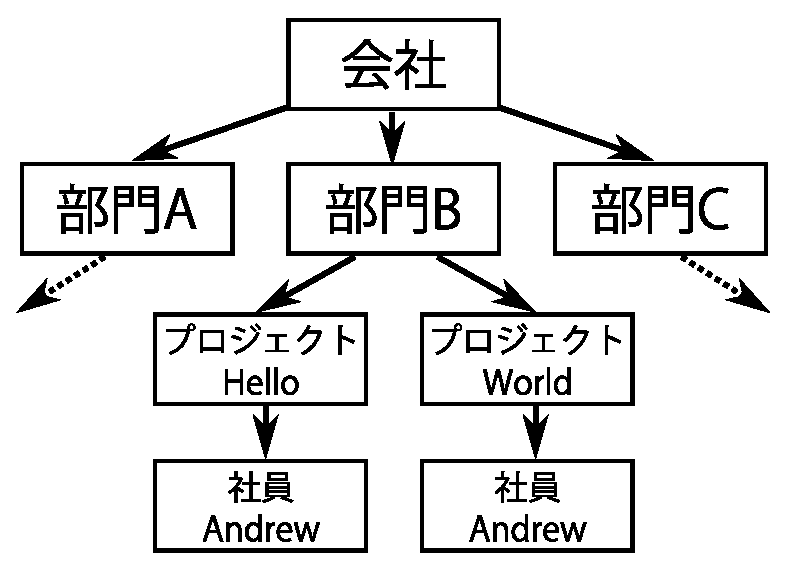
\includegraphics[width=5cm]{hayamiz/images/hierarchical-data-model.eps}
   \caption{階層型データモデル}
   \label{214539_12Jul12}
  \end{center}
 \end{minipage}
 \begin{minipage}{0.48\textwidth}
  \begin{center}
   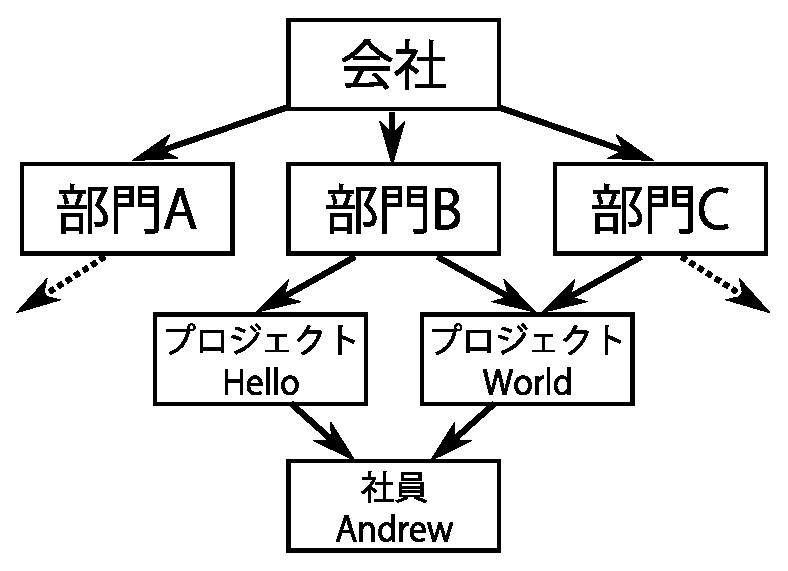
\includegraphics[width=5cm]{hayamiz/images/network-data-model.eps}
   \caption{ネットワーク型データモデル}
   \label{214707_12Jul12}
  \end{center}
 \end{minipage}
\end{figure}

階層型データモデルというのは、木構造を用いてデータを組織化したデータモデ
ルです。たとえば会社組織を階層型データモデルで表そうと思うと、会社の下に
は複数の部門が属しており、各部門の下には複数のプロジェクトがあり、各プロ
ジェクトの下には社員が属している、というようにスキーマを定義してゆきます
(図\ref{214539_12Jul12})。ここで、例えば2つのプロジェクトHelloとWorldに属
する1人の社員Andrewがいたとしたらどうでしょう。階層型データモデルでは、あ
るデータの実体(ここでは1人の社員)は親となるデータの実体(プロジェクト)
を複数持つことができません。そのため、各プロジェクトごとにAndrewのデータ
を持つことになり、データの重複が生じてしまいます。また、部門Bと部門Cが共
同でプロジェクトWorldを運営していることを表現しようと思うと、プロジェクト
のデータに加えてその下にぶら下がっている社員のデータも併せてコピーしなけ
ればなりません。このような欠点を克服したのがネットワーク型データモデルで
す(図\ref{214707_12Jul12})。ネットワーク型データモデルでは、データの実
体が複数の親を持つことができる有向グラフをデータ構造として採用したため、
前述のようなデータ重複の問題は発生しません。

ネットワーク型モデルによりより一般的なデータ構造を表現できるようにはなり
ました。しかし、階層型モデルやネットワーク型モデルに基づくデータベースは、
データのアクセスに一つ大きな問題を抱えていました。これらのデータベースに
おいてデータの問い合わせを行う際には、データの構造がどのようになっている
かを把握し、そしてどのような手順でデータを取得するかを利用者が知っている
必要があったのです。例えば図\ref{214707_12Jul12}のデータベースにおいて社
員Andrewのデータを取得するためには、「会社のデータを読みとり、部門Bのデー
タを読み取り、プロジェクトHelloのデータを読み取り、社員Andrewのデータを読
み取る」という手順を指定してあげなければなりません。このように、欲しいデー
タにアクセスするための``how'' をもって問い合わせを行うデータベースシステ
ムは、ユーザがデータの案内(navigation)をするという意味で{\bf ナビゲーショ
ナルデータベースシステム}と呼ばれます。

もしもナビゲーショナルデータベースシステムにおいて、図
\ref{214707_12Jul12}の会社で組織改変があり、各部門の下には課が設置され、
その下にプロジェクトが属するという構造にデータベースが修正されたとしたら
どうなるでしょう。これまで社員のデータにアクセスするアプリケーションは会
社→部門→プロジェクト→社員とたどっていましたが、会社→部門→課→プロジェ
クト→社員とたどるように修正しなければなりません。このように、ナビゲーショ
ナルデータベースシステムでは、ある特定のデータのみに興味があったとしても、
その上位構造に変化があった時にはデータにアクセスする方法を再構成しなけれ
ばなりませんでした。当時IBMはIMSという階層型データモデルにもとづくデータ
ベースシステムを開発していましたが、IMSを使ったシステムではデータ構造の変
更に伴うコードのメンテナンスにほとんどの時間を吸い取られていました。

歴史的には、階層型モデルはそのシンプルさ故に初期のデータベースシステムに
おいて採用され、その後により一般的なデータの組織化を行うことができるよう、
ネットワーク型モデルが発明されます。1969年にはCODASYLという委員会によって、
ネットワーク型データモデルの標準化が行われ、データベースシステムの情勢は
階層型モデルからネットワーク型モデルに移るかと思われました。

そこに登場したのが、1970年\footnote{正確にはリレーショナルデータモデルの
論文は1969年にIBMの社内技術報に掲載され、翌1970年に米国コンピュータ学会の
論文誌に掲載されます。}にCoddによって提唱されたリレーショナルデータモデル
です。リレーショナルデータモデルでは、データの論理的な構造と物理的な構造
が独立しているため、データ構造を変更するたびにアプリケーションを書き直す
必要がありません。また、ユーザは「どんなデータが欲しいか」を記述するたけ
で、具体的なアクセス方法はデータベース側が判断してデータを取得することが
できます。つまり、ナビゲーショナルデータベースシステムでは ``how'' を与え
なければデータのアクセスが行えなかったのですが、リレーショナルデータベー
スは ``what'' を与えるだけでデータのアクセスが可能となります\footnote{リ
レーショナルモデルの数学的な定義や、なぜそれにより``what''でデータの問い
合わせが可能となるのかの説明については、それだけで一冊の本になってしまう
ので他書に譲ります。}。

また、リレーショナルモデルは集合論にもとづくしっかりとした数学的基礎の上
に成り立っており、後のデータベースシステム研究の大きな基盤となりました。
これまでプログラマによるある種の職人芸の上に成り立っていたデータベースシ
ステムは、リレーショナルデータモデルの登場によって科学の領域へと押し上げ
られたのです。

\section{INGRESプロジェクト始動}

リレーショナルデータモデルがCoddによって提唱されてから3年が経った1973年が
終わろうとする頃、その論文が一人の若き研究者の目に留まりました。その人こ
そ、INGRESプロジェクト、そして後のデータベース業界全体を率いる存在となる
Michael Stonebraker です。1971年にミシガン大学で博士号を取得し、UC
Berkeleyで研究職についたばかりのStonebraker はテニュアトラック
\footnote{テニュアとは大学における終身雇用資格のことです。若手研究者は任
期の限られた研究職につき、テニュア獲得を目指して研究業績を積み上げてゆく、
というの米国における一般的な研究者のキャリアパスです。このテニュア獲得の
ための若手研究者が通る道をテニュアトラックと呼びます。テニュアトラックで
いかに論文を``量産''できる研究ネタを選ぶかというのは、若手研究者にとって
は人生に関わる重要な決断なのです。}を走り始めたばかりであり、何か良い研究
のネタはないかと思案していたところでした。そんな Stonebraker にとって、リ
レーショナルモデルは恰好の研究対象だったのでしょう\footnote{ちなみに
Stonebraker の博士論文は ``The Reduction of Large Scale Markov Models
for Random Chains'' というタイトルで、もともとは数学寄りの研究をしていた
ようです。 }。リレーショナルデータモデルに出会った Stonebraker は、
Eugene Wong と共にリレーショナルデータベースシステムの実装に乗り出します。
こうしてINGRESプロジェクトは始まりました。

% http://genealogy.math.ndsu.nodak.edu/id.php?id=31091

INGRESという名前は、{\bf IN}teractive {\bf G}raphic and {\bf RE}trieval
{\bf S}ystem の頭文字をとったもので、本来は UC Berkeley の経済学の研究チー
ムのために、地理情報をグラフィカルに表示するためのシステム研究として予算
を獲得していたプロジェクトでした。そこは本音と建前で、まずはデータを効率
的に取得するためのデータベースシステムが必要だ、ということで Stonebraker
達はデータベースシステムの開発にのめりこんでゆきます。

こうして走り始めたINGRESプロジェクトですが、データベースシステムを動かす
ためのコンピュータはありませんし、そもそも Stonebraker や Wong は大きなプ
ログラム開発の経験すらありませんでした。リレーショナルデータベースシステ
ムの先駆けであるINGRESは、まさにゼロからのスタートでした。

何はなくともデータベースシステムの開発環境がなければ話になりません。
INGRESプロジェクトが始まって Stonebraker が最初に取り組んだのは、コンピュー
タの調達と開発環境作りでした。当時といえば、データベースシステムを構築す
るためには高価なメインフレームを導入して、COBOLでプログラムを書くという時
代でした。リレーショナルデータベースシステムのように、まだ世の中に存在す
らしていないソフトウェアのために、研究職になりたての Stonebraker がメイン
フレームを手に入れることができるわけもありません。

そんな中、ミニコンピュータと呼ばれる、いわゆる現在のPCの先駆けとなる安価
なコンピュータシステムが1960年代に生まれ、そして1970年代にはミニコンピュー
タをビジネスに活用しようという動きが高まり、小型ビジネスコンピュータ市場
が生まれました。時を同じくして、ベル研究所では Ken Thompson 達によってミ
ニコンピュータ上で動作する汎用オペレーティングシステムUNIXの開発プロジェ
クトが始まりました。UNIXはもともとアセンブリで実装されていましたが、
Dennis Ritchie 達によってUNIX開発のためにC言語が開発され、1973年にはC言語
に移植されました。そう、まさにINGRESプロジェクトが始まったその年です。

Stonebraker は開発環境として UNIX を、そしてINGRESの実装言語としてC言語を
使うことを決めます。そして UNIX が動作するコンピュータとして選ばれたのが、
DECのPDP-11/70でした。UNIXが最初にベル研究所以外の場所でインストールされ
たのがこのINGRESプロジェクトであり、インストール時には Ken Thompson と
Dennis Ritchie が5MBのディスクを抱えてやってきたそうです。

\section{INGRESの進化}

INGRESプロジェクトでは、リレーショナルデータベースシステムの実装における
重要な技術が多数生み出されてゆきました。当時のINGRESがどのように設計され
ていたのか、1976年に発表された論文``The design and implementation of
INGRES''をもとに、その技術的な側面を概観してゆきます。

\begin{center}
 \begin{minipage}{0.95\textwidth}
  \begin{screen}
   以降の説明で使われる用語

   \footnotesize
   \term{リレーション}{リレーショナルデータモデルにおける、いわゆ
   るテーブルのこと}

   \term{タプル}{リレーショナルデータモデルにおける、いわゆるレコードの
   こと}

  \end{screen}
 \end{minipage}
\end{center}

\subsection{クエリ言語QUELとEQUEL}

リレーショナルデータベースでは、それ以前のナビゲーショナルデータベースと
は異なり、どんなデータが欲しいか``what''を記述するだけで、具体的にどのよ
うなデータ構造やアルゴリズムが実装されているかを一切知る必要なくデータを
取得することができる、というのが大きなウリの一つです。その``what''を記述
するための言語がクエリ言語です。皆さんのよく知っているSQLもクエリ言語の一
つです。

INGRESプロジェクトでは、クエリ言語としてQUELが開発されます。リレーショナ
ルデータモデルに併せて Codd はDSL/APLHAというクエリ言語を1971年に発表して
いるのですが、DSL/ALPHAは数学的な表記\footnote{DSL/ALPHAは関係演算
(relational calculus)をベースとして、量化子$\exists, \forall$や、論理演算
の記号$\lnot,\land,\lor$などがほぼそのまま用いられいていました}に基づいて
おりやや一般的にわかりやすいものではありませんでした。QUELはDSL/ALPHAをベー
スとして、数学的な表記のない``やさしい''クエリ言語として設計されました。

QUELがどんな言語なのか、簡単なサンプルコード\footnote{1975年のINGRESの論
文より引用}をみてみましょう。

\begin{center}
 \begin{minipage}{0.9\textwidth}
  \begin{verbatim}
RANGE OF C IS CITY
RETRIEVE INTO W(C.CNAME,
                DENSITY = C.POPULATION / C.AREA)
         WHERE C.STATE = 'California'
           AND C.POPULATION > 50000
  \end{verbatim}
 \end{minipage}
\end{center}

このサンプルコードでは、カリフォルニア州にある人口5万人以上の市について、
市の名前と人口密度の一覧を取得するという処理を行っています。一行目の
RANGE文では、処理の対象としてCITYリレーションを選択して、CITYリレーション
のタプルを表す変数名Cを宣言しています。二行目のRETRIEVE文は、SQLでいうと
ころのSELECT文に相当します。処理の結果は、一時テーブルとして作成されるWに
保存されます。細かい表記の違いを別にすると、現在使われているSQLとそれほど
大きな違いがないことがわかると思います。

\subsection{アクセスメソッドとデータ構造}

アクセスメソッドとは、その名前の通りデータベースに保存されているデータに
アクセスするための方法です。例えば、とある会社の従業員のデータがEMPリレー
ションに1万人分保存されていたとします。この中から、ある従業員1人分のタプ
ルを取り出すには、どうすればよいでしょうか。もっともナイーブには、EMPリレー
ションを頭から全部スキャンして、目的の従業員のタプルを探すという方法が考
えられます。これも立派なアクセスメソッドの一つですが、1人分のデータを探す
にはちょっと効率が悪すぎます。従業員番号でタプルを並べておいて、二分探索
するというやり方も簡単に思いつく方法です。これもアクセスメソッドの一つと
いえます。

アクセスメソッドには様々な実装方法があり、それぞれが得意とするデータアク
セス、苦手とするデータアクセスのパターンがあります。データベースシステム
のように総合的なデータの管理を行うためのシステムでは、複数のアクセスメソッ
ドを利用できる必要があります。

\subsubsection{アクセスメソッドインターフェース}

INGRESには、複数のアクセスメソッドを利用するためのインターフェースが
定められています。INGRESで標準的に提供されるアクセスメソッドはすべてこの
インターフェースを介して提供されており、またこのインターフェースに従って
実装することで独自のアクセスメソッドを追加することができるように設計され
ています。

INGRESで定められているアクセスメソッドインターフェースは次の通りです:
\begin{enumerate}
 \item {\bf OPENR}({\it descriptor}, {\it mode}, {\it relation\_name})
 \item {\bf GET}({\it descriptor}, {\it tid}, {\it limit\_tid}, {\it
       tuple}, {\it next\_flag})
 \item {\bf FIND}({\it descriptor}, {\it key}, {\it tid}, {\it key\_type})
 \item {\bf PARAMD}({\it descriptor}, {\it access\_characteristics\_structure})
 \item {\bf PARAMI}({\it index\_descriptor}, {\it access\_characteristics\_structure})
 \item {\bf INSERT}({\it descriptor}, {\it tuple})
 \item {\bf REPLACE}({\it descriptor}, {\it tid}, {\it new\_tuple})
 \item {\bf DELETE}({\it descriptor}, {\it tid})
 \item {\bf CLOSER}({\it descriptor})
\end{enumerate}
{\bf OPENR} と {\bf CLOSER} はプログラマにとってはファイル操作等でお馴染
みの関数でしょう。{\bf OPENR} で指定したリレーションを開き、リレーション
のディスクリプタを取得します。以降、このリレーションに対するアクセスはこ
のディスクリプタを以って行われます。一連のアクセスが完了した後は、{\bf
CLOSER} によってリレーションを閉じます。

{\bf GET} は、タプルID(tid)をキーとしてタプルのデータを取得するための関数
です。{\it tid}でタプルIDの下限を、{\it limit\_tid}でタプルIDの上限を指定
することができ、{\bf GET}が呼び出されるとこの条件にマッチする最初のタプル
を見つけてきて、そのデータを {\it tuple} に書き込みます。また、{\it
next\_flag}にTRUEを指定して{\bf GET}を呼び出した場合には、次にマッチする
タプルのIDを{\it tid}に書きこむため、連続してタプルを読みだしてゆくことが
できます。

{\bf FIND}は、{\it key}で指定した検索キーにマッチするタプルIDを取得するた
めの関数です。{\it key\_type}で完全一致検索、範囲検索などの検索モードを指
定することができます。

{\bf PARAMD}、{\bf PARAMI}は{\bf FIND}において利用可能な検索キーの種類や、
検索モードを調べるための関数です。それぞれ、データファイル用と、索引ファ
イル用に利用されます。

{\bf INSERT}はタプルを挿入するための関数、{\bf REPLACE}は既に存在するタプ
ルを更新するための関数、{\bf DELETE}はタプルを削除するための関数です。

\subsubsection{データ構造}

INGRESでは、{\bf ヒープ}、{\bf ハッシュ}、{\bf ISAM}、{\bf 圧縮ハッシュ}、
{\bf 圧縮ISAM}の5種類のアクセスメソッドが提供されています。

{\bf ヒープ}は単純にタプルを並べてゆくだけの最も単純な構造で、タプルを探すとき
は毎回線形探索を行います。非常にタプル数の少ないリレーションや、クエリの
実行結果を格納する一時的なリレーションに適しています。

\begin{figure}[tb]
 \begin{center}
  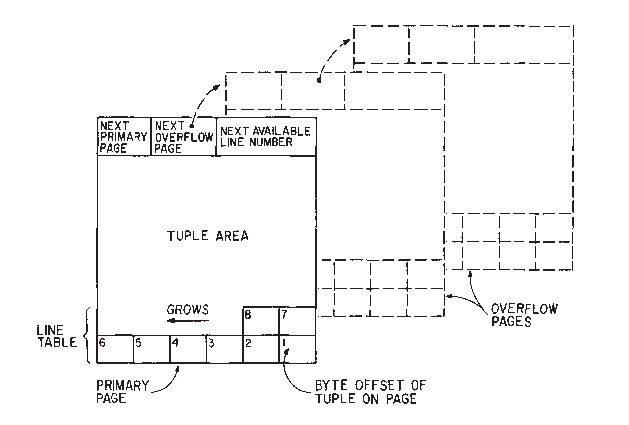
\includegraphics[height=66mm]{hayamiz/images/page-layout-ingres.eps}
  \caption{INGRESのページ構造}
  \label{174456_16Jul12}
 \end{center}
\end{figure}

{\bf ハッシュ}と{\bf ISAM}は、検索キーを用いて少量のタプルに対するアクセ
スを高速に行うことを可能とする構造です。{\bf ハッシュ}はハッシュテーブル
を使って、{\bf ISAM}は探索木を使って、検索キーとタプルIDの関連付けを行う
ことで、高速なアクセスを実現しています。INGRESでは、タプルIDは (ページ番
号, ページ内ライン番号) という値のペアによって表現されているので、タプル
IDさえわかれば目的のデータの在り処がわかります。

ページの構造は図\ref{174456_16Jul12}のようになっています。ページの先頭に
はヘッダ情報があり、またページの末尾にはラインテーブルと呼ばれるデータが
格納されています。ラインテーブルの各要素は、タプルのデータがページ内のど
の位置にあるかのオフセット情報を保持しています。タプルIDに含まれているペー
ジ内ライン番号は、このラインテーブル内のインデックス番号となっているので、
タプルIDさえわかればタプルのデータがどこにあるのかがわかるようになってい
ます。この構造には、タプルの物理的な位置が変化しても、ラインテーブルを更
新するだけで、タプルIDは変化することがないという利点があります。

\subsubsection{アクセスメソッドまとめ}

\begin{figure}
 \begin{center}
  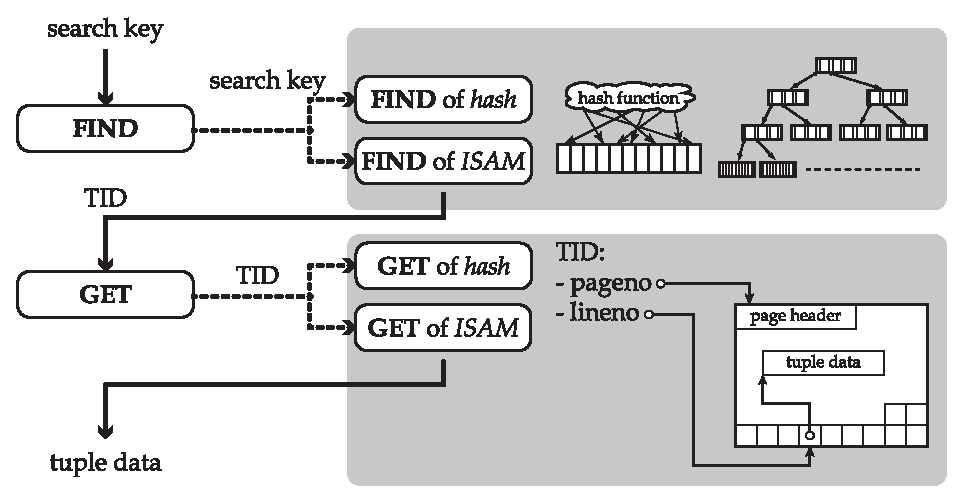
\includegraphics[width=100mm]{hayamiz/images/access-method.eps}
  \caption{検索キーを用いたアクセスメソッドによるタプルデータの取得}
  \label{190817_16Jul12}
 \end{center}
\end{figure}

検索キーが与えられてから、タプルのデータが得られるまでの一連の流れを図
\ref{190817_16Jul12}にまとめました。まずは検索キーが与えられると、{\bf
FIND}を呼び出してタプルIDを取得します。{\bf FIND}の中では、ハッシュテーブ
ルや木構造を用いて効率的にタプルIDの検索が行われます。そして、得られたタ
プルIDを引数として{\bf GET}を呼び出すことで、ページを読み出し、タプルのデー
タが取得されます。

この基本的なデータアクセスの枠組みは、INGRESの頃に確立され、現在でも殆ど
変わること無く引き継がれています。

ただ1980年頃まで、INGRESには B$^+$-tree を用いたアクセスメソッドは実装さ
れていませんでした。ISAMとB$^+$-treeはよく似ているのですが、根本的な違い
としてISAMは静的なアクセスメソッドであるのに対し、B$^+$-treeは動的なアク
セスメソッドであるということです。どちらも多分木構造を索引として用いてい
ますが、ISAMではデータの挿入や削除のたびに木構造を変更することはなく、適
当なタイミングでまとめて木構造を作り直します。そのため、頻繁にデータの挿
入、削除が行われる場合にはどんどん構造劣化が進み、アクセス性能が落ちてし
まいますが、参照が非常に多い場合には良い性能を発揮します。一方、
B$^+$-treeはデータの挿入、削除のたびに木構造を動的にバランスさせるために、
ISAMで起きるような構造劣化は起きません。しかし、1回の処理あたりのオーバー
ヘッドはISAMよりも大きくなってしまいます。

INGRESの開発において、何度もB$^+$-treeの導入が検討され、その度に採用が見
送られてきたようです。しかしながら、1980年のINGRES開発を振り返る論文にお
いて、StonebrakerはB$^+$-treeの採用を見送ってきたのは ``major mistakes''
の一つであり、次にアクセスメソッドを再検討する際にはB$^+$-treeも実装する
であろうと述べています。

また、INGRESのアクセスメソッドはUNIXのファイルシステムの上に構築されてい
たのですが、UNIXのファイルシステムによるオーバーヘッドが当初予測していた
よりも深刻なものであり、独自のファイルシステムを実装するべきであった、と
も同論文では述べられています。実際に、3年後に発表された論文において
Stonebraker 達は独自に実装したファイルシステムを使った場合と性能比較を行っ
ており、最大で70\%程度性能が向上することを確認しています。このように
INGRESの開発過程で得られた知見は、UNIXの開発にもフィードバックされ、その
発展にも大きく貢献しました。

\subsection{クエリ処理エンジン}

\section{System R}

INGRESプロジェクトからすこし遅れて、IBMでもリレーショナルデータベースシス
テム System R の研究開発が始まります。リレーショナルデータモデルの父であ
る Codd はIBMで働いていたにも関わらず、歴史を振り返るとIBMはリレーショナ
ルデータベースシステム開発において常に後塵を拝しています。

TODO:

\section{エピローグ}

1970年代には、Coddによるリレーショナルデータモデルの提唱に始まり、INGRES
やSystem Rの研究によってリレーショナルデータベースシステムが実用に耐えう
るものであることが証明されました。1981年には、Coddはその功績が認められ計
算機科学分野において最も権威ある賞であるチューリング賞を受賞します。

そして1970年代の終盤から1980年代は、商用リレーショナルデータベースシステ
ムが次々と登場し、熾烈な戦いを繰り広げてゆきます。

1977年、現在の Oracle の前身である Software Development Laboratories が
Larry Ellison と Robert Miner によって設立され、1979年にはSQLベースの商用
リレーショナルデータベースシステムとしては世界初となる Oracle RDBMS の発
売を開始します。

1979年、Jack Shemer、Philip Neches、Walter Muir、Jerold Modes、William
Worth、Carroll ReedによってTeradataが設立され、1984年には世界初の並列デー
タベースシステムDBC 1012をリリースします。

1980年、Lawrence Rowe、Michael Stonebraker、Eugene Wong、Gary
Morgenthaler によって INGRES 商用化のために Relational Technology (後の
Ingres Corp.)が設立され、翌1981年に最初の商用INGRESをリリースします。

時を同じくして、Roger Sippl と Laura King によって 1980年に Relational
Database Systems (後の Informix Software) が設立され、翌1981年に
Informix がリリースされます。

IBMは1981年にSQL/DSを、さらに1983年にはDB2をリリースしてリレーショナルデー
タベース市場に乗り出します。エンタープライズ市場の覇者であるIBMのこの動き
は、旧来のナビゲーショナルデータベースシステムに対する新興勢力リレーショ
ナルデータベースシステムの勝利を決定的なものにします。

1984年、Mark Hoffman、Bob Epstein、Jane Doughty、Tom Hagginによって
Sybaseが設立され、1986年にリレーショナルデータベースシステムSybaseをリリー
スします。後にSybaseはMicrosoftと提携してSybase SQL Serverを開発し、その
設計はMicrosoft SQL Serverにも受け継がれています。

同1984年、ミニコンピュータ市場を牽引するDECがOpenVMSオペレーティングシス
テムにおける機能として DEC Rdb を発表します。

1986年、無停止コンピュータシステムを主な事業として手がける Tandem
Computers が NonStop SQL をリリースします。

そして1990年代には更にプレイヤーが増えつつもその統廃合が進み、オブジェク
ト指向データベースシステムなど進行技術の登場、オープンソースのデータベー
スシステム隆盛の兆候など、データベースシステムは新たな時代へと突入してゆ
きます。

\section*{参考文献}

\small

\begin{itemize}
 \item E. F. Codd, ``A Relational Model of Data for Large Shared Data
       Banks'', {\it Communications of the ACM}, Volume 13, Number 6,
       1970
 \item E. F. Codd, ``A data base sublanguage founded on the relational
       calculus'', {\it Proceedings of the 1971 ACM SIGFIDET workshop
       on Data Description, Access and Control}, 1971
 \item C. J. Date, E. F. Codd, ``The relational and network approaches: Comparison of the
       application programming interfaces'', {\it Proceedings of the
       1974 ACM SIGFIDET workshop on Data Description, Access and
       Control}, 1975
 \item G. Held, M. Stonebraker, E. Wong, ``INGRES--A relational data
       base management system'', {\it Proceedings of AFIPS 1975 NCC},
       Volume 44, 1975
 \item M. Stonebraker, G. Held, E. Wong, P. Kreps, ``The design and
       implementation of INGRES'', {\it ACM Transactions on Database
       Systems}, Volume 1, Issue 3, 1976
 \item G. Held, M. Stonebraker, ``B-trees re-examined'', {\it Communications of the
       ACM}, Volume 21, Issue 2, 1978
 \item M. Stonebraker, ``Retrospection on a database system'', {\it ACM
       Transactions on Database Systems}, Volume 5, Issue 2, 1980
 \item D. Chamberlin, M. Astrahan, M. Blasgen, J. Gray, W. F. King,
       B. Lindsay, R. Lorie, J. Mehl, T. Price, F. Putzolu, P. Selinger,
       M. Schkolnick, D. Slutz, I. Traiger, B. Wade, R. Yost, ``A
       history and evaluation of System R'', {\it Communications of the
       ACM}, Volume 24, Issue 10, 1981
 \item M. Stonebraker, J. Woodfill, J. Ranstrom, M. Murphy, M. Meyer,
       E. Allman, ``Performance enhancements to a relational database
       system'', {\it ACM Transactions on Database Systems}, Volume 8,
       Issue 2, 1983
 \item Relational Technology Inc., ``INGRES The Distributed SQL
       Relational Database System Press Kit'', 1987
 \item National Research Council, ``Funding a Revolution: Government
       Support for Computing Research'', Natl Academy Pr, 1999
 \item M. Stonebraker, J. M. Hellerstein, ``What Goes Around Comes
       Around'', {\it Readings in Database Systems, Fourth Edition},
       Morgan Kaufmann, 2005
 \item A. Ances, ``RDBMS Workshop: Ingres and Sybase'', Computer
       History Museum, 2007
\end{itemize}

and so many online resources

\normalsize
% -*- coding: utf-8 -*-

\chapter{PostgreSQLカンファレンス2012 レポート}

\begin{flushright}
 {\headfont はやみず}
\end{flushright}

2012年3月24日に日本PostgreSQLユーザ会主催で開催されたPostgreSQLカンファレ
ンス2012に参加してきました。この記事は、PostgreSQLカンファレンス全体の概
観についてレポートを記したものです。

このカンファレンスはオフィシャルサイトにあるように技術的な話題を中心とし
て、PostgreSQLに関する導入事例や技術的な話題を提供するためのカンファレン
スです。 昨年度の参加者約180名に対して今年度は275名(関係者含む)ということ
で、日本におけるPostgreSQLのユーザ層の広がりを感じさせます。 特にこの数年
はビジネスとしてこのカンファレンスに参加する方も増えているそうで、業務用
途としてのPostgreSQLの利用が広まっていることを示しているのではないかと思
われます。

Linuxの急速な普及をきっかけとして、今やオープンソースソフトウェアを業務に
おいて利用することは全く珍しくなくなっています。 PostgreSQLもその例に漏れ
ず、といったところでしょうか。本年度のカンファレンスのプログラムも、業務
用途におけるPostgreSQLの利用ということが一つの大きな軸として捉えられてい
るように見えます。 例えば、午後のプログラムは3トラック構成となっていたの
ですが、そのうちの1トラックは「マイグレーショントラック」と題して他の
DBMSからPostgreSQLへ移行することを主眼としたものであり、「商用 DB から
PostgreSQL への移行」「PostgreSQL がより使いやすく進化した Postgres Plus
Advanced Server の実力とは」などは明らかに商用DBを意識しています。また、
技術トラックやLightning Talkにおいて高可用・高性能なPostgreSQLクラスタに
関する発表がありました。業務用DBMSとしてはクラスタソリューションがほしい。
MySQLにはMySQL Clusterが、OracleにはOracle RACが、じゃあPostgreSQLはどう
なの?というポイントに答えを出すのが、今回のカンファレンスの一つの見所だっ
たのではないでしょうか。

もちろん、ビジネス的な側面だけではなく、技術の深い話もできるのがこのカン
ファレンスの魅力だと思います。午前中の基調講演では、PostgreSQLの大型移行
案件の事例紹介であるフランス社会保障機構の講演に加えて、PostgreSQLのコア
開発者でありコミュニティの中でも若手のエースと目されているEnterpriseDB社
のRobert Haas氏によるPostgreSQL 9.2の新機能に関する講演がありました。こち
らの講演では、メニーコア環境におけるスケーラビリティ向上の取り組みや、
Index-only Scanの導入、消費電力削減のための実装努力、レプリケーションの新
機能、その他細々とした新機能などが紹介されました。加えて、バージョン9.2よ
り後にどんな技術的な課題に取り組んでいくべきか、といった方向性についても
触れられていました。質疑応答も非常に活発に行われていたのが印象的です。一
つ残念だったのは、こちらの講演は発表・質疑応答ともに逐次翻訳が行われてい
たため、実際に話せる時間が半分になってしまっていたことです。英語のみで進
行してくれたほうが個人的には中身がもっと詰まって面白かったのではないかと
思いますが、難しいところですね。

もう1件技術的な講演として面白かったのは藤井雅雄氏、松尾隆利氏による
「PostgreSQL 9.1 同期レプリケーションと Pacemaker による高可用クラスタ化
の紹介」です。 こちらの発表では、まず藤井氏からPostgreSQLにおけるレプリケー
ションの詳細について紹介されていました。非同期レプリケーション、同期レプ
リケーションの動作や、何ができるのか、何ができないのかについて丁寧にまと
められており、レプリケーション機能の全体像を理解できる発表でした。またそ
れに加えて、9.2で導入される予定のレプリケーション関連の機能紹介や、周辺ツー
ルに関する紹介もありました。 その後、松尾氏により同期レプリケーション機能
とPacemakerを組み合わせることによる、障害発生時にもフェイルオーバ可能なク
ラスタ構成法についての発表が行われました。Pacemakerについては名前くらいし
か知らなかったのですが、障害発生からフェールオーバまでの流れがわかりやす
く図解されており、Pacemakerを知るという観点からも有用な発表であったように
思います。

本会議のほうについてはこんなところで、懇親会にも参加したのでの話をひとつ。
PostgreSQLのお役立ち情報源として参照している人も多いかと思われるLet's
Postgresという読み物サイトがあるのですが、こちらの運営をしている方とお話
をさせて頂きました。 この手の読み物サイトでは、最も需要の高い入門系記事や、
企業の提灯記事が並ぶというのがよくあるパターンなのですが、Let's Postgres
にはPostgreSQLの内部構造についてやたら詳しく書かれた記事がたくさんあり、
これは一体どういったことだろうと思っていたのでした。 そのことを聞いてみた
ところ、内部構造の多くは記事PostgreSQL本体にコミットしている開発者の方々
が好きで寄稿しているということだそうです。PostgreSQL自体が内部構造まで含
めた子細なドキュメントが充実していますが、新機能の実装詳解がこれほどまで
精力的に行われているソフトウェアはなかなかないのではないかとおもいます。
これらの記事は目的別ガイド:内部解析編としてまとめられています。内部の詳
解に加えて、開発プロセスへの参加方法についても紹介されており、非常に充実
した内容となっています。PostgreSQLの中身に興味がある人は必見ですね。

以上、簡単ではありますが参加レポートでした。

% TODO: もっと書く


% -*- coding: utf-8 -*-
%!TEX root = ../book.tex

%\cleardoublepage
%\plainifnotempty

\chapter{とある世界で一番高速なBrainfuckインタプリタ}
\begin{flushright}
hogelog
\end{flushright}

\section{まえがき}
\lettrine{世}
の中にはたくさんのプログラミング言語が存在します。
Dennis RitchieはUnixを記述するためにC言語を作り
\footnote{The Development of the C Language* 
\verb|http://cm.bell-labs.com/cm/cs/who/dmr/chist.html|
},
Tecgrafチームはブラジルの貿易障壁の影響下で
Luaを
\footnote{
The Evolution of Lua
\verb|http://www.lua.org/doc/hopl.pdf|
},
そしてUrban M\"ullerは
チューリング完全な最小限の言語として
Brainfuckを作成しました
\footnote{
\verb|http://www.muppetlabs.com/~breadbox/bf/|
}
。

世の中にはたくさんのプログラミング言語処理系が存在します。
例えばRuby言語には
まつもとゆきひろによるオリジナル実装を元にした
MRI\footnote{
\verb|http://www.ruby-lang.org/ja/|
},
JVM上で動作する
JRuby\footnote{
\verb|http://jruby.org/|
},
JITコンパイラや世代別GCなどが組み込まれた
Rubinius\footnote{
\verb|http://rubini.us/|
},
組み込みスクリプトエンジン向けとして作られた
mruby\footnote{
\verb|https://github.com/mruby/mruby/|
}
など様々な処理系があります。
例えば大規模分散処理のためHadoopフレームワークを利用したければ
JRubyを使うこともあるでしょう。
エディタアプリケーションにスクリプト機能を組み込むためにはmrubyを
使うかもしれません。
言語処理系にとって重要な機能は
使う局面によって変わってきますが,
処理系が高速であればだいたいの人は嬉しいでしょう?

Brainfuckという言語は
\verb|+ - > < , . [ ]|
という8個の命令しか存在しない,
処理系の実装が容易な言語です
\footnote{
\verb|http://www.kmonos.net/alang/etc/brainfuck.php|
とかわかりやすい解説だと思います
}。
以下ではBrainfuckインタプリタの高速化を通じて
\textbf{インタプリタの高速化}
技術について親しんでいきましょう。
とりあえずはこの記事のタイトル通りに
{\Large \textbf{世界で一番高速なBrainfuck処理系}}
を作ってみましょう。

なお以下で示すサンプルコードは
筆者のgithubリポジトリ
\footnote{\verb|https://github.com/hogelog/sample-code/tree/master/dbtimes-vol01|}
から適宜参照できます。

\section{普通の処理系}
{\scriptsize
\verb|https://github.com/hogelog/sample-code/blob/master/dbtimes-vol01/bf.cpp|
}

さて,まずはなんの高速化も施されていない
Brainfuck処理系を実装します。
(図\ref{bf.cpp})

たったこれだけの記述で一応ちゃんとした
言語処理系になるんだから楽で良いですね。

\begin{figure}[hbt]
\begin{minipage}{0.5\hsize}
{\scriptsize
\begin{verbatim}
#include <stdio.h>
#include <string>
int main() {
  std::string code;
  for (int ch;(ch=getchar())!=EOF;)
    code.push_back(ch);
  static int membuf[30000];
  int *mem = membuf;
  int depth = 0;
  for (size_t pc=0;pc<code.size();++pc) {
    switch(code[pc]) {
      case '+': ++*mem; break;
      case '-': --*mem; break;
      case '>': ++mem; break;
      case '<': --mem; break;
      case ',': *mem = getchar(); break;
      case '.': putchar(*mem); break;
      case '[':
\end{verbatim}
}
\end{minipage}
\begin{minipage}{0.5\hsize}
{\scriptsize
\begin{verbatim}
        if (*mem == 0) {
          depth = 1;
          while (depth != 0) {
            switch(code[++pc]) {
              case '[': ++depth; break;
              case ']': --depth; break;
            }}}
        break;
      case ']':
        depth = -1;
        while (depth != 0) {
          switch(code[--pc]) {
            case '[': ++depth; break;
            case ']': --depth; break;
          }}
        --pc;
        break;
    }}
  return 0;
}
\end{verbatim}
}
\end{minipage}
\caption{
普通のBrainfuckインタプリタ
}
\label{bf.cpp}
\end{figure}

\section{インタプリタ高速化}
上述したインタプリタは簡潔ですしちゃんと動くので良いのですが
あまり高速ではないので,
いくつかの高速化を施して世界最速インタプリタにしてみましょう。

\subsection{VM化}
{\scriptsize
\verb|https://github.com/hogelog/sample-code/blob/master/dbtimes-vol01/bf-vm.cpp|
}

プログラムの文字列を逐次解釈するインタプリタを
高速化する手法として,
プログラムをVM\footnote{Virtual Machineの略}
命令列へ変換する部分と
VM命令列のインタプリタ部分に分ける方法がよく知られています。
RubyインタプリタのMRIは
バージョン1.9から
独自VMを内蔵するようになり,
大幅な高速化に成功しました。
ここではBrainfuckインタプリタの
VM化を試してみましょう。

図\ref{bf.cpp}
のプログラムは
\verb|[ ]|命令を処理する部分に
while文があるのが気になります。
\verb|[|
と対応する
\verb|]|
は一度調べればわかるのに,
毎回1文字ずつ探すのは効率がよくありません。
\verb|[ ]|命令
を対応するVM命令の位置を保持するVM命令へと
変換することで,
\verb|[ ]|命令
の処理部分から
while文が消えます。
(図\ref{bf-vm.cpp:loop})

またプログラムを実行するforループで毎回
\verb|pc<code.size()|
とチェックするのも無駄です。
処理するVM命令列の最後に
「処理を終了する」命令を一つ追加することで,
終了判定もswitch文の中に混ぜることができました。
(図\ref{bf-vm.cpp:finish})

\begin{figure}[hbt]
\begin{minipage}{0.3\hsize}
{\scriptsize
\begin{verbatim}
struct Instruction {
    char op;
    int jmp;
};
\end{verbatim}
}
\caption{
VM命令構造
}
\label{bf-vm.cpp:structure}
\end{minipage}
\begin{minipage}{0.3\hsize}
{\scriptsize
\begin{verbatim}
case '[':
    if (*mem == 0) {
        pc = code.jmp;
    }   
    break;
case ']':
    pc = code.jmp;
    break;
\end{verbatim}
}
\caption{
[]命令処理部分
}
\label{bf-vm.cpp:loop}
\end{minipage}
\begin{minipage}{0.3\hsize}
{\scriptsize
\begin{verbatim}
    for (size_t pc=0;;++pc) {
        Instruction code = codes[pc];
        switch(code.op) {
            ...
            case '\0':
                return;
\end{verbatim}
}
\caption{
終了処理
}
\label{bf-vm.cpp:finish}
\end{minipage}
\end{figure}


\subsubsection{direct threaded code}
{\scriptsize
\verb|https://github.com/hogelog/sample-code/blob/master/dbtimes-vol01/bf-vm2.cpp|
}

VMの高速化手法の一つに
direct threaded code
と呼ばれる手法があります。
詳細は
Ruby 1.9
のVM化を主導した
笹田耕一さんによる記事
YARV Maniacs
\footnote{\verb|http://jp.rubyist.net/magazine/?0008-YarvManiacs|}
に任せますが,
この手法により
命令処理部分に存在した大きな
switch文による分岐コストを
大幅に軽減できます。

\subsection{JITコンパイル}
{\scriptsize
\verb|https://github.com/hogelog/sample-code/blob/master/dbtimes-vol01/bf-jit.cpp|
}

前の章ではVM化として
プログラムをVM命令に変換する部分と
VM命令を処理する部分に分けることによる
最適化について説明しました。
しかしどうせ変換するなら
プログラムを実際の機械語列に変換して,
その機械語列をそのままCPUに実行してもらえば
良いのです。
この手法はJITコンパイルと呼ばれています。
最近では各種ブラウザベンダが
「うちのブラウザのJavaScriptエンジンはJITコンパイラを内蔵してるから速いんだ!」
と主張しあってたりすることから
耳にする機会も多いでしょう。

Xbyak\footnote{
\verb|http://homepage1.nifty.com/herumi/soft/xbyak.html|
},
asmjit\footnote{
\verb|http://code.google.com/p/asmjit/|
}
などのJITアセンブラを
用いると,
各命令処理をアセンブラ相当の記述をするだけで
JITコンパイラができますし,
慣れてしまえば簡単ですね?

\subsection{最適化}
\begin{figure}[hbt]
{\scriptsize
\begin{verbatim}
+++++++++++++[->++>>>+++++>++>+<<<<<<]>>>>>++++++>--->>>>>>>>>>+++++++++++++++[[
>>>>>>>>>]+[<<<<<<<<<]>>>>>>>>>-]+[>>>>>>>>[-]>]<<<<<<<<<[<<<<<<<<<]>>>>>>>>[-]+
<<<<<<<+++++[-[->>>>>>>>>+<<<<<<<<<]>>>>>>>>>]>>>>>>>+>>>>>>>>>>>>>>>>>>>>>>>>>>
>+<<<<<<<<<<<<<<<<<[<<<<<<<<<]>>>[-]+[>>>>>>[>>>>>>>[-]>>]<<<<<<<<<[<<<<<<<<<]>>
>>>>>[-]+<<<<<<++++[-[->>>>>>>>>+<<<<<<<<<]>>>>>>>>>]>>>>>>+<<<<<<+++++++[-[->>>
>>>>>>+<<<<<<<<<]>>>>>>>>>]>>>>>>+<<<<<<<<<<<<<<<<[<<<<<<<<<]>>>[[-]>>>>>>[>>>>>
>>[-<<<<<<+>>>>>>]<<<<<<[->>>>>>+<<+<<<+<]>>>>>>>>]<<<<<<<<<[<<<<<<<<<]>>>>>>>>>
[>>>>>>>>[-<<<<<<<+>>>>>>>]<<<<<<<[->>>>>>>+<<+<<<+<<]>>>>>>>>]<<<<<<<<<[<<<<<<<
<<]>>>>>>>[-<<<<<<<+>>>>>>>]<<<<<<<[->>>>>>>+<<+<<<<<]>>>>>>>>>+++++++++++++++[[
>>>>>>>>>]+>[-]>[-]>[-]>[-]>[-]>[-]>[-]>[-]>[-]<<<<<<<<<[<<<<<<<<<]>>>>>>>>>-]+[
\end{verbatim}
}
\caption{とある巨大なBrainfuckプログラム(抜粋)}
\label{mandelbrot.b}
\end{figure}
\begin{figure}[hbt]
{\scriptsize
\begin{verbatim}
c[->cmc>c>+m]mc>cmc[[m]+[m]m-]+[mz>]m[m]mz+mc[-[-m+m]m]m+m+m[m]mz+[m[mzm]m[m]mz+
mc[-[-m+m]m]m+mc[-[-m+m]m]m+m[m]m[zm[m[-m+m]m[-m+m+m+<]m]m[m]m[m[-m+m]m[-m+m+m+m
]m]m[m]m[-m+m]m[-m+m+m]mc[[m]+>z>z>z>z>z>z>z>z>zm[m]m-]+[
\end{verbatim}
}
\caption{とある巨大なBrainfuckプログラム(抜粋)を最適化}
\label{mandelbrot.b:opt}
\end{figure}

{\scriptsize
\verb|https://github.com/hogelog/sample-code/blob/master/dbtimes-vol01/bf-vm-opt.cpp|
}

{\scriptsize
\verb|https://github.com/hogelog/sample-code/blob/master/dbtimes-vol01/bf-jit-opt.cpp|
}

ここまでは対象言語を問わない汎用的な高速化手法を紹介しました。
ここからはBrainfuck特有の性質に着目した最適化を施してみましょう。

図\ref{mandelbrot.b}
のプログラムをしばらく眺めてみると,いくつかの無駄が存在することに気づきます。
まずは
\verb|++++|,
\verb|----|,
\verb|>>>>|,
\verb|<<<<|
のような同じ命令の繰り返し。
{\it n}個の
\verb|+|命令
の繰り返しは
{\it n}加算する
\verb|c|命令,
{\it n}個の
\verb|-|命令
は
{\it -n}加算する
\verb|c|命令に置き換えられます。
同様に
\verb|>|
と
\verb|<|
も
\verb|m|
命令に
置き換えられます。

またよく出てくる命令の組み合わせに
\verb|[-]|
があります。
これは「メモリの値が0になるまで\verb|-|命令を繰り返す」という処理,
つまり「メモリの値を0にする」という
\verb|z|命令
に
置き換えてしまいましょう。

ここまでの最適化で
図\ref{mandelbrot.b}
のプログラムが
図\ref{mandelbrot.b:opt}
までに圧縮されます。
特に
\verb|z|命令
の導入により,
存在していたループ処理のいくつかが消えています。

このように,あとはひたすら
「こういう組み合わせよく出てくるからこういう特定の命令に置き換えよう」
という作業を続けるだけで,なんと世界で最速のBrainfuckインタプリタが
完成したのでした
\footnote{
\verb|https://github.com/hogelog/fast-bf|
}。

「世界最速の処理系だ」と主張しているのに,
まだ誰も「こっちの方が速い」
と言ってこないので,たぶん世界最速なんじゃないかな。
たぶん。きっと。おそらく。
% -*- coding: utf-8 -*-
%!TEX root = ../book.tex

\cleardoublepage
\plainifnotempty

\chapter{クラウド時代のDNS}
\begin{flushright}
suu-g
\end{flushright}

%\section{Welcome to DNS world}
\lettrine{ヰ}
ンターネットが始まってから20年、ARPANETから数えると40年以上。
インターネットはここ十年ほどで一気に生活に不可欠のものとなりました。
そんなインターネットを支える基礎技術の一つがDNSです。

そんなDNSを取り巻く状況ですが、今年は随分と熱い一年間でした。
DNSの最初のRFC 1034, 1035 が出たのは1987年でしたが、それから25年
経過した今でもなお新たな問題が発覚し続ける、枯れているようで
枯れていない少し枯れた技術DNS。その現状と問題を、プロトコルを
確認しながら追っていくのがこの記事です。

とはいえ、普通のソフトウェア屋さんにとってDNSとは使うものであって
それ以外ではないのでしょうから、こちらの世界のニュースについては
あまり確認されていないことと思います。

今年は、どんなことが起きたのでしょうか?
DNS界隈で起きた問題について羅列してみます。
\begin{itemize}
  \item (日本)児童ポルノに関するDNSブロッキング立法・ISPにおける運用が開始
  \item SOPAにGo Daddyが賛成を表明するも一日で撤回
  \item SOPAに反対を表明するためWikipediaが24時間閉鎖する
  \item SOPAに反対を表明してAnonymousがOperation Blackoutを表明
  \item フレッツ網におけるIPv6-IPv4フォールバック問題の解決法として、国内各所でAAAAフィルタリングが検討される
  \item Google, AAAAフィルタを導入している可能性のあるDNSサーバに対してAAAAレコードを回答しない運用を宣言
  \item 浸透言うな!
  \item Ghost Domain問題の発表
  \item ニフティクラウドのDNS障害問題
  \item GMOクラウドのDNSで謎の障害がある
  \item さくらのDNSに(サブ)ドメインジャッキングが可能な脆弱性が発覚
  \item JPRSがあらためてコンテンツサーバとキャッシュサーバの兼用の危険性を告知
  \item BIND, 長さ0のRDATAにより異常終了する脆弱性(重複をお許しください)
  \item お名前.com、ninja toolsのNSレコードを規約に基づき変更
  \item 今年の夏のDNS祭りはBINDではなくNSD
\end{itemize}

豊作ですね。
問題に限定しなければ他にも、DNSSEC.jpが活動を終了したり、
gTLDの申請があったりと、今年は本当に色々なことがありました。

今回は、「クラウド」時代となった今、DNS界隈でどのような
問題が起きているかを振り返ります。

\section{DNSとぼくらの世界}

DNSのパケットフォーマットは、RFC1034,1035 に載っている通りです。
DNSパケットには四つのセクションがあり、それぞれQuery, Answer, Authority,
それからAdditionalと呼ばれています。
\footnote{http://www.ietf.org/rfc/rfc1034.txt Section 3-7}
\footnote{http://www.ietf.org/rfc/rfc1034.txt Section 4-1}
それぞれのセクションに入ったデータの意味を適切に解釈することで、DNSの
メッセージ伝達は動作しています。

これをJSON風に書くと、図1のようになってます。(正確には、DNSSECやEDNS0対応
等でフラグはもう幾つかある)
読者の皆様におかれましてはこのパケットの意味を判断しようとしてくれると
期待しますが、勘の良い人だと、このプロトコルのもつ怪しさをなんとなく
感じ取ったかも知れません。

さて、このようなパケットを元にして、DNSというシステムは成り立っています。
このパケットを用いて Paul Vixie らが作ろうとしたのが、巨大な名前空間の木です。
そして、その木をデータベースとしてユーザから参照できるようにした。それが
DNSというシステムです。あ、ご存知ですよね。すいません。でも大事なこと
なんで。

ここでnoteしておきたいのが、DNSプロトコルが作られた当時の時代情勢です。
DNSは、/etc/hostsからの移行のひとつの可能性として生まれていたわけですが、
その時代が今とは違っていて、例えばDNSでちょっと間違いが起こったとしても、
それは手動で直していれば良かった。今じゃ警察沙汰だもん。もぉーちょっと
お名前.comさん。NS勝手に向けないでー。

もっとも、DNSに関しては今でも法的にきちんとしているとは言い難いところです。
DNSでのブロッキングの効果を法律で認めているわりには、JPRSが電気通信事業者
というわけでもありませんし。このあたりは、そろそろ本格的に議論されるべき
話ですよね。

さて話は戻ります。いま当時の時代情勢を取り上げたのは、DNSという
分散システムが、設計段階から「異なる管理者同士で」ひとつの巨大な名前空間を
管理するように作られている、ということを再認識したかったからです。
各管理者が責任を持つ名前空間の範囲をゾーンと呼び、その空間の管理を他の人に
任せることを委譲と呼んでいる。そういう信頼関係となっています。
それらを前提として、内容に入って行きましょう。


\section {DNSの正常系}

DNSの正常系は、先に示しました4つのセクションと5つのフラグを使い、
おおよそ次の5種類のパケットを用います。
\begin{enumerate}
  \item Query (recursive)
  \item Query (not recursive)
  \item Response (Authoritative, with glue record in additional section)
  \item Response (with Answer)
  \item Response (against recursive query)
\end{enumerate}
非常にフリーダムです。

ユーザがキャッシュサーバに対して問い合わせを行い、そのキャッシュサーバ
がユーザの代わりにイテラティブにクエリを発行するときのパケットは、
図のようになります。

キャッシュサーバがキャッシュを持ったあとは、1と5のパケットのみの
やりとりとなります。ここまでは皆様ご存じですねー。

また、このキャッシュサーバがコンテンツサーバも兼ねている場合、
図のようなレスポンスが返ってくることになります。
ユーザからは、これはAAビットが立って(権威のある回答として)見えます。
なお、権威のある回答は通常のキャッシュと比較して優先されるべき
ものということになっていますが、ユーザには大差ありません。
\footnote{http://www.ietf.org/rfc/rfc2181.txt}

正常系としては、こんなところでしょう。これだけの機能があれば、
ルートサーバを頂点とする綺麗なツリー構造が世界に作れます。
すばらしい!DNS最高!いあ!いあ!


\section { 異常系 }
以上のようなDNSですが、問題が山積みです。これはどう考えても
プロトコルが悪いのです。

\subsection{ Lame Delegation }
これは基本だよなあ。基本が火を噴くか否か、そこのスリルを味わってみたいなあ。
要は、上位のサーバでの正しくない設定です。
責任者の違いはありますが、構造的には、 Visaドメイン問題 
\footnote{http://www.e-ontap.com/summary/}
と言われているものもこれのうちのひとつと数えてしまって良いでしょう。


\subsection{ 浸透さんって幽霊じゃね? }

DNSの設定変更や引っ越しをしたときに、その結果が「浸透」
するのを待たなければいけない…というのは有名な嘘ですが、
その「浸透」現象自体は実際に起こっていて、それもサーバ
の実装バグのせいだった、と言うことが最近分かりました。
\footnote{www.isc.org/files/imce/ghostdomain\_camera.pdf}
これが「幽霊ドメイン」です。 
具体的な問題内容については、DNSOpsの資料 
\footnote{http://dnsops.jp/bof/20120425/20120425-DNSOPS.jp-BoF\_Ghost\_Domain\_Names\_v02.pdf}
や「Geekなぺーじ」
\footnote{http://www.geekpage.jp/blog/?id=2012/3/21/1} に詳しい
のでそちらをご参照ください。

ソフトウェア的に考えたときに問題となるのは、古いキャッシュ
が残存して昔のサーバへ問い合わせを続けるということ、
それから、問い合わせを続けていると古いキャッシュがexpire
しないという実装バグがあったということ。そして最後に、
本来のDNSのツリーから外れたコンテンツサーバが、レコードを
消さずに残しているために、昔のレコードをいつまでも返し続ける
場合があるということ。この三点です。

本来の信頼関係から外れたところのデータが有効性を持ってしまい、
おまけにその状態を意図的に作り出せる、という状態ですね。
このような問題が今年までバグとして存在し続けていたわけです。

システムとして考えると、キャッシュをTTL分保持することは
至極もっともなようですが、信頼関係のツリーまで含めてキャッシュすると
いうことは、非常に責任が大きい行為です。
今回のように、「なぜかキャッシュが消えない」という
異常事態になったとき、影響が大きくなります。


\subsection{ サブドメインジャッキング問題 }
2011年6月、さくらのDNSサービスにおいて、一時的にサブドメイン
ジャッキングが可能になっていた問題が発覚しました。
これは、 example.jp ドメインが登録されていたとしても、別のユーザに
よって自由に www.example.jp ドメインを作成できてしまった、という
問題です。
\footnote{さくらはたまたま注目を浴びただけで、問題を抱えたサービス
プロバイダは他にもたくさんある…が、その話はまた今度}

これは、DNSの本質的な問題を幾つか激しく突いています。

ひとつには、DNSの作成しているツリーが理想的なものではないこと。
あるゾーンを委譲する先のサーバは、別ホストになっているとは限らず、
同じホストである可能性があります。
そのため、フルリゾルバが正しく委譲されている先のサーバにたどり着く
前に、どこかの「ゾーンを持っていると勝手に宣言している」だけの
サーバによって偽の情報を掴まされる可能性があります。

ふたつめとして、ゾーンと言う概念が、プロトコルや実装とかけ離れて
しまっているという点があります。
ドメインのデリミタはドットですが、ドットがあったからと 言って
ゾーンが違っているかどうかは不明です。
example.jp ゾーンを他へ委譲したサーバ上で www.example.jp のAレコードを
登録できなくなるわけではありませんし、www.example.jpを問い合わせた
ときにどちらが返って来るかは実装依存(!) になってしまっています。


最後に、フルリゾルバがどのコンテンツサーバにも同じクエリを投げる、
というプロトコルの怪しさがあります。
これは、どこでゾーンが分かれるかが問い合わせを行うまでは
キャッシュサーバには知ることができない、ということとは符合します。
しかし、キャッシュサーバはゾーンの別れ方について【知らないでは済まされない】。
問い合わせを行ったキャッシュサーバは即座にその結果をキャッシュする
ことを実際に行っています(RFC的には、「キャッシュしても良い」)。
キャッシュサーバは、一種類の問い合わせを行ったときの結果によって、
様々な動作を行います。これは、最終的にコンテンツを持っているサーバから問い合わせる
ために用いるパケットも、そのサーバを見つけるためのパケットも同じということで、
それらの違いはフルリゾルバが判断する必要があります。
どうせキャッシュサーバは状態を持つのだから、結果を見て処理をディスパッチ
するよりも、メッセージやパケットフォーマットや通信の口を変えた方が、
圧倒的に楽でバグが少なくなったでしょうね。

もしも問い合わせがゾーンごとに行われていれば、子ゾーンについて問い合わせて
いるところで孫ゾーン情報が返ってきたり、あるいはAレコード問い合わせ
に対して謎のNSレコードをキャッシュさせられたりすることは無かったでしょう。
どう見てもプロトコル上の脆弱性です。本当にありがとうございました。

これらの問題点を合わせて起こった問題が、このサブドメインジャッキング問題です。


\subsection{ キャッシュ兼用サーバ }
コンテンツ・キャッシュ兼用サーバはしばしば問題と言われます。
先に示したように、自由に偽ドメインを入れられるコンテンツサーバを
フルリゾルバとして使用するのは、 自分のホストの /etc/hosts の書き換え権を
他人に委ねているようなものだ、というのはお分かりいただけるかと思います。

さて、ソフトウェア的に見た時に、キャッシュ兼用サーバに潜むDNSの問題は
というと…、これは優先順位やレイヤの問題があります。
AuthoritativeなサーバからのAnswerセクションは、他のどのレコードよりも
優先されるべきだとRFC2181にありますが、毒入れの可能性を考えたときに
もっとも危険性が高いのも、このAuthoritativeなAnswerセクションです。
このりくつはおかしくない。

「DNSサーバの相乗りという業務形態自体が、プロトコルとの相性が悪いのではないか」
と言った方がいましたが、 その意味が分かるのではないでしょうか。


\section{まとめ}
DNSは今やインターネットに不可欠な存在となっていますが、大きな問題があります。
その問題をEDNS0やDNSSECなどを用いて解決しようとしているのが現在のDNS界隈
ですが、そもそもDNSというプロトコル自体に設計レベルでの問題が多すぎます。
皆様方におかれましては、このDNSという「想定外に利用されてしまった」
プロトコルの問題を他山の石とし、これからの分散システムの開発にぜひ
活かしていただければ、記事を書いた当人としては満足でございます。

以上、タイトル詐欺の記事でした。おあとがよろしいようで。


% -*- coding: utf-8 -*-


\chapter{IPv4がこの先生きのこるには}
% * (アスタリスク)付きの \chapter* コマンドは原則不可とする

\begin{flushright}
 yuyarin % ペンネーム
\end{flushright}

\section{はじめに}

\lettrine{イ}
ンターネットの主要技術であるIPv4というプロトコル.その中で個体識別子として使われるIPv4アドレスは32bitで表現され数は約42億個である.
かつては「無限アドレスだぜヒャッハー」と湯水のように消費されていたのだが,70億もの人間が社会インフラとしてインターネットを必要としている
今となっては,このアドレスの数が全く足りなくなってしまっているのだ.
レジストリから事業者へのIPv4アドレスの新規割り振りはほぼ終了しており,IPv4アドレスは「枯渇」したと表現されている.

この枯渇を見越して作られた次世代プロトコルがIPv6である.IPv4の失敗を踏まえて色々な改良は施されているが,なんといっても128bitのアドレス空間が魅力である.
国内主要ISPのバックボーンは既にIPv6に対応できており,一部のISPでは利用可能になっているが,中小ISPや地方CATV,ICP\footnote{Internet Content Provider}ではまだ対応できていない.

1998年にRFC2460にてIPv6の仕様が発表されてから既に14年が経っているのだが,未だにほんの一部にしか普及していないのだ.
ISPは通信相手のICPがIPv6に対応していなければ対応する必要性は薄いし,
ICPもほんの一部のISPの一部のユーザしかIPv6を使えないのに対応するのは金がかかるだけなのだ.
デッドロックに陥っているのだ.

さすがにこのままではダメだということで,2012年6月6日にはWorld IPv6 Launchとして,
Googleを筆頭に世界中の主要サイトがIPv6を恒久的に有効にするという取り組みが行われた.
こうして徐々にデッドロックが解けてIPv6への対応が進んでいき,IPv4アドレスの枯渇問題がそれを更に加速させるだろう.
そしてIPv6が主要のプロトコルになりIPv4は古の技術として扱われるようになる未来が来るだろう.

だがしかし,すべての通信がIPv6に対応できるまで,我々はアドレスが枯渇しているIPv4を必死に「延命」させなければならないのだ.

前置きが長くなったが,この章ではそんな「IPv4延命技術」を紹介しようと思う.

\section{IPv4延命技術概観}

枯渇によってIPv4アドレスの割り振りを受けられなかったISPにおいて,顧客に割り当てるIPv4グローバルアドレスが
無くなってしまうというシナリオが,今後実際に起こるだろう.というか起きてる.
この時に必要になるのは\textbf{顧客間でIPv4グローバルアドレスを共有する}方法である.
IPv4アドレスの共有にはNAT\footnote{実際にはNAPTだが以降NATと呼ぶことにする}が使われる.

主要な延命技術をNATの場所とIPv4パケットの運び方で分類した表を表\ref{yuyarin-nat-transport}に示す.

\begin{table}[htbp]
\begin{center}
\begin{tabular}{c|ccc} \hline
 & IPv4ネイティブ & \multicolumn{2}{c}{IPv6トランスポート} \\
 & & カプセル化 & トランスレーション \\\hline
CPEでNAT & いまここ & MAP-E(旧4rd) & MAP-T(旧dIVI) \\
ISPでNAT & CGN & DS-Lite & 464XLAT \\\hline
\end{tabular}
\end{center}
\caption{NATの場所とトランスポート方法によるIPv4延命技術の分類}
\label{yuyarin-nat-transport}
\end{table}

\subsection{IPv4ネイティブ方式}

現在のIPv4ネットワークではCPE\footnote{Customer Premises Equipment},いわゆるご家庭のルータでNATをしている.
これも1家庭(CE\footnote{Customer Edge})で1アドレスを共有するという1つのアドレス節約術であり,実は既にこの延命戦は始まっていたのだ.
これに更にISP側でNATを重ねることで複数の家庭で1つのグローバルアドレスを共有するのがCGN(Carrier Grade NAT)である\footnote{表ではISPでNATとしているが,実際にはCPEとISPの両方でNATを行うことになる}.

\subsection{IPv6トランスポート方式}
それに対してCPEにIPv6アドレスを割り当て,そのIPv6を利用してISP網内のIPv4バックボーンまでIPv4パケットを通す方法がある.
これはIPv6の使い方によってカプセル化とトランスレーションに分けられる.
カプセル化はいわゆるトンネルのことで,CPEとISPの間でIPv4 over IPv6トンネルを張り,IPv4パケットをIPv6パケットのデータとして運ぶ.
トランスレーションではIPv4パケットをIPv6区間を通る間だけIPv6パケットに変換する.

\begin{figure}[htbp]
 \begin{minipage}{0.5\hsize}
  \begin{center}
   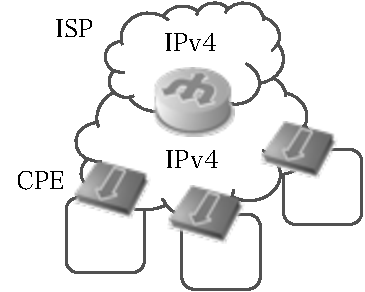
\includegraphics[bb=0 0 175 140,width=40mm]{./yuyarin/cgn.pdf}
  \end{center}
  \caption{IPv4ネイティブ}
  \label{fig:one}
 \end{minipage}
 \begin{minipage}{0.5\hsize}
  \begin{center}
   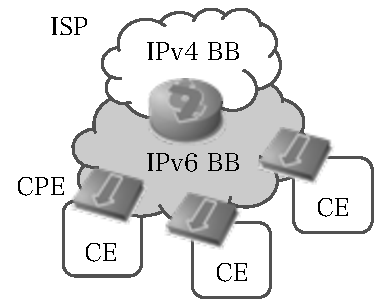
\includegraphics[bb=0 0 175 140,width=40mm]{./yuyarin/v6transport.pdf}
  \end{center}
  \caption{IPv6トランスポート}
  \label{fig:two}
 \end{minipage}
\end{figure}

これらは更にNATをする場所によって分類できる.

CPEで特殊なNATをして,プライベートアドレスからグローバルアドレスへ変換した後,
IPv6でカプセル化するのがMAP-E(旧4rd),IPv6へトランスレーションするのがMAP-T(旧dIVI)である.
MAPにおけるNATの特殊性は外部送信元ポートとして利用されるポート番号が各CPEで限定されることである.

プライベートアドレスのIPv4パケットをIPv6でカプセル化してISP網内へ運んだ後,ISP側でNAT(CGN)してグローバルアドレスへ変換するのがDS-Lite(Dual Stack Lite)であり,
プライベートアドレスのIPv4パケットをIPv6パケットにトランスレーション(NAT46)して,ISP側でNAT(NAT64)するのが464XLATである.

これらの技術においてIPv4グローバルアドレスは複数のCEで同じ物が共有される.いくつのCEで共有するかが設計のパラメータとなる,だいたい目安としては256程度である.

\section{ステート管理のお話}

\subsection{CGNのNATの問題}

NATの根底にある設計思想はアドレスだけでは識別子が足りないのでポート番号も識別子に使ってしまおうというものである.
NATでは(内部アドレス,内部送信元ポート,外部アドレス,外部送信元ポート)というバインディングをセッション情報として一定期間保持している.
そうしないと外から戻ってきたパケットを内側の誰に送って良いのかわからなくなるからである.

CGNでは何千という家庭の通信をNATしなくてはならないので,NATのセッションデータベースは巨大なものになり生成頻度も高くなる.
ISPはユーザの通信を最低限90日間は保存しなくてはならないのだが,この時にNATのデータベースも併せて保存しておかないと
通信元の顧客が特定できなくなってしまう.

これらの処理はソフトウェアで行う必要があるため,ネットワーク機器からすれば意外と重い処理なのだ.
顧客数を$n$とすると定数項が大きい$\mathrm{O}(n)$の仕組みなのだがネットワーク業界ではこれはスケールすると言わなかったりする.

\subsection{IPv6トランスポート方式でのCPE特定の問題}

DS-Lite以外のIPv6トランスポート方式ではISPからCPEへIPv4パケットを送ろうとした時に,
どのIPv6アドレスのCPEに対してパケットを送るのかを特定しなければならない.
NATに非常によく似た状況であるのだが,IPv6のアドレスの長さを生かした工夫がされている.

MAPではIPv4アドレスとポート番号が決まればIPv6アドレスが相互に一意に定まるような「ルール」を決めてアドレス変換を行う,
Stateless Address Mapping(SAM)という方式を採用している.
ルールさえ各機器で共有してしまえばCPEを特定するためのデータベース(ステート)の管理をする必要がないのだ.
464XLATではRFC6145のStateless IP Translationを行なっており,こちらもステートを持たない.

この仕組みは顧客数nに対して定数オーダー$\mathrm{O}(1)$で処理できるために良くスケールする.
ISP側に置く設備1つに対して帯域が許す限り多くのCPEを収容しても問題ないのだ.

\subsection{ISP側NATにおける可用性の問題}

\begin{figure}
\centering
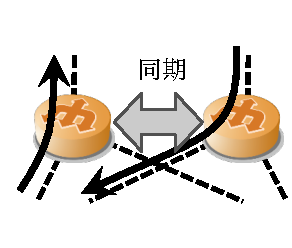
\includegraphics[bb=0 10 140 109,width=5cm]{./yuyarin/cgn-nat.pdf}
\caption{行きと帰りで違う箱を通るパケットと必死で同期するNAT箱}
\end{figure}

ISPでは当然ネットワークの冗長性を確保しなくてはならない.
ISP側でNATする技術については,2台の巨大NAT箱を置かなくてはならないのだ.

Act-Standby構成の場合,故障した時に即座にStandby機を起動して故障した機器からNATのセッションデータベースを受け取らなくてはならない.
故障しているのにそのようなことはできるはずがないので,当然ながらAct-Act構成になる.

IPネットワークでは往路と復路が必ずしも一致しない.NAT箱1を通って出ていったパケットの応答がNAT箱2に戻ってくることは,当たり前に起こりうることである.
よって2台のNAT箱は常にNATの巨大なセッションデータベースを同期し続け無くてはならないのだ.

もちろん非常に大変な処理なのだが,そこは力技でなんとかする感じである.

\section{結局どの技術がイケてるのか?}

\subsection{CGN}
スケールもしないし泥臭いので技術的には大変な割にダサい.
でも既存の家庭用ルータには手を入れずにISPに設備を置くだけでよい.
ハイスペックな機器があって,収容するCPEの数を上手に設計して,その分お金をかければなんとかなるのかもしれない.

\subsection{MAP-E(4rd), MAP-T}
MAPは技術的な面では非常にイケている.
ステートレスなアドレス変換を行うため定数オーダーでスケールところが非常に素晴らしい.

カプセル化をする場合はMTUの問題とフラグメントの問題が発生する.
実装面での負荷は高いが既存のMAP(4rd)実装ではこの点を既にクリアしている.
トランスレートする場合はIPv4の属性がIPv6に変換された時点で失われてしまう.

しかしながらデプロイが非常に難しい.
NTTのホームゲートウェイやBuffaloやNECのルータなど家庭用ルータにMAPの複雑な実装を入れなくてはならない.
ビジネス的な視点で見るとこれがとてつもなく高価になってしまうのだ.

\subsection{DS-Lite}
ISPでNATするのでCGN同様にスケーラビリティはない.
CPEにも機能を入れなくてはいけない.
あまりイケてない.

\subsection{464XLAT}
ステートフルトランスレーション(RFC6146)とステートレストランスレーション(RFC6145)の組合せで作られていて非常に美しい.
NAT64に始まるトランスレーション技術の最終形態とすら思える.

しかしやはりISP側でNATをしてステートを持ってしまうためスケールしない.
また各家庭のCPEに機能を追加する必要が出てくる.
今のところCPE(CLAT)ではNEC-ATなどの実装がある.
ISP側の機器(PLAT)はNAT64のため既に多くのベンダで実装が行われている.

\section{おわりに}

技術的にはMAPや464XLATがイケてるのだけれども,ビジネス的な面ではCGNでないとデプロイできないだろう.
とはいっても今回の記事で紹介したのはひとつの切り口であって,他にも語れなかった要素があるので,
他の技術も活躍できる場所が多いにあるのだ.結局は適所適材なのである.

アプリケーションを開発する人には,今後このように家庭間でのアドレス共有ということがISPで行われることを知ってもらいたい.
もはやIPアドレスだけでは誰かを特定できないのだ.
1つのIPアドレスでのBANが何千世帯に対して影響することが今後起こりうるのだ.
2ちゃんねるでプロバイダごとアク禁を食らったかのようなことが,いとも容易く起きてしまうのだ.

アドレスが枯渇したIPv4を我々はこのようなアドレス共有技術を用いてちまちまと延命していかなくてはならない.
自律分散システムであるがゆえに,地デジのように「今日でアナログ放送は終わりです」ということはできない.

IPv4はこの先生きのこらなければならず,そのためにはこうした技術や仕組みを考えて,標準化して,
製品に組み込んで,設計をして,お金をかけてリアルなインターネットにデプロイしなくてはならないのだ.

とっくの昔から,インターネットが止まると人が死ぬ時代になってしまっている.
ネットワークオペレータの戦いは終わらない.


% -*- coding: utf-8 -*-

\chapter{プログラマ的同人誌執筆環境構築概論}
% * (アスタリスク)付きの \chapter* コマンドは原則不可とする

\begin{flushright}
 はやみず
\end{flushright}

\lettrine{技}
術者たるもの、同人誌を書く時であってもその技術的ノウハウを積極的に投入し
て、執筆作業を最大限に効率化しなければならない。そのような信条のもとに、
本誌の執筆環境は構築された。

% \vspace*{2mm}
% 
% \begin{center}
%  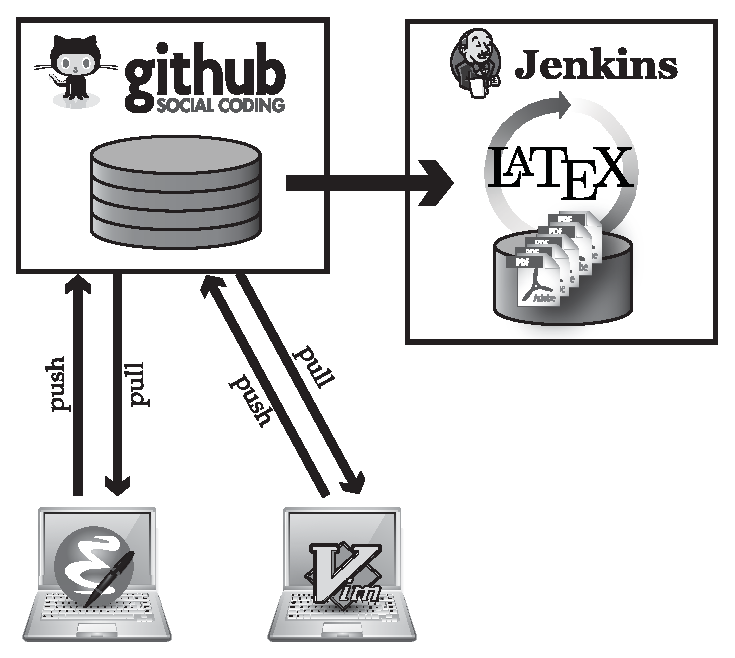
\includegraphics[width=8cm]{hayamiz/images/dbtimes-env.eps}
% \end{center}

\section{LaTeX}

文章執筆はLaTeXに限る。

% 文章ファイルの保存形式は、やはりプレインテキストでなければならない。最近
% はWordも構造化された文章を執筆するための機能が整いつつあるという。しかし
% ながら、我々はプログラマである。プログラマは、各自の研ぎ澄まされたテキス
% トエディタ環境を有している。即ち、執筆速度を最大化するためには、各々が最
% 大限能力を発揮できるテキストエディタ環境を利活用することが最善である。そ
% のためには、やはりプレインテキストでなければならない。

文章ファイルの保存形式は、やはりプレインテキストでなければならない。プロ
グラマは各自の研ぎ澄まされたテキストエディタ環境を有している。即ち、執
筆速度を最大化するためには、各々が最大限能力を発揮できるテキストエディタ
環境を利活用することが最善である。そのためには、やはりプレインテキストで
なければならない。

そして、我々プログラマは情報を構造化されていない状況に極度のストレスを覚
える生き物である。ある程度以上の長さ、内容の高度さをもつ文章を執筆する場
合には、図表や章・節の参照、文献管理、目次の作成、整合性のある文章スタイ
ル調整など、文章全体が高度に構造化され、文章内の要素が有機的に結合されて
いなければならない。これを為すためには、高度かつ柔軟な組版システムを利用
することが必要不可欠である。

やはり、文章執筆はLaTeXに限る。

本誌の組版には \TeX Live 2011 を用いてる。文書のクラスには奥村先生の
{\tt jsbook.cls} を利用しており、{\tt tombow} オプションを利用することで
トンボ付きの出力を得ている。{\tt tombow}オプションを利用する際には、併せ
て{\tt papersize}オプションを利用しないと、文書のサイズとしてはトンボ無し
で出力されてしまうので注意が必要である。

\section{GitHub}

文章執筆はGitHubに限る。

複数名で共同作業を行う場合、最近では Dropbox が用いられる場合が多い。
Dropbox は便利である。一度導入してしまえば、誰でも簡単にファイルを即時に
共有することができる。

しかし、我々はプログラマである。プログラマは変更履歴を重んじる生き物であ
る。即ち、バージョン管理システムはプログラマにとって必須である。Dropboxに
も履歴管理機能は存在するが、限定的でありインターフェースも非効率なもので
ある。

また、プログラマは編集の競合に注意を払う生き物である。特に本誌のように締
切のあるようなものの場合、締切直前には多数の編集が競合することが予想され
る。Dropbox では、競合の解決をシステマティックに行うことは不可能である。
一方、バージョン管理システムはその基本機能として競合解決のシステマティッ
クな方法を提供する。バージョン管理システムに高いリテラシを有する我々にとっ
て、これを用いないことは有り得ない。

そして今日、GitHubはプログラマの共通基盤である。殆どのプログラマは、各々
のSSH公開鍵をGitHubに登録済みである。即ち、GitHubをバージョン管理システム
のホストとして用いることで、最小限の手間で共同作業基盤を構築可能である。

幸いなことに、私はGitHubのプライベートレポジトリを作成できるアカウントを
保有している。そのため、原稿はクローズドな形で管理することが可能である。

やはり、文章執筆はGitHubに限る。

\section{継続的インテグレーション}

文章執筆は継続的インテグレーションに限る。

我々は重要な事実に目を向けなければならない。\LaTeX の基盤たる \TeX という
言語は、単なるマークアップ言語にあらず。チューリング完全性を有する、完備
なるプログラミング言語であり、\LaTeX による文章執筆とは即ちプログラミン
グ行為であり、ソフトウェア開発にほかならないのである。

ソフトウェア開発において、今日最も重要視されている開発基盤の一つが継続的
インテグレーションである。バージョン管理システムにコードがコミットされる
度に、プログラムがビルドされ、テストコードが走り、常に最新の成果物が生成
された状態が維持される。一度誤ったコードがコミットされた折には、そのこと
が開発者に直ちに通知され、更なる状況の悪化を食い止めるフィードバックルー
プを形成する。

% また、\LaTeX による文章執筆における特有の問題として、最終成果物であるPDF
% ファイルに正しくフォントを埋め込むための環境構築には一定の手間を要すると
% いうことがある。執筆者全員が、あまねく必要なフォントをすべて保持し、適切
% に \LaTeX 環境を設定することは難しい。必要なフォントを持たない場合には、
% 代替フォントによって文章をプレビューする他にない。一方で、継続的インテグ
% レーションのためのビルドサーバにおいてこのような環境を構築しておけば、執
% 筆者全員が最終成果物を正しい形で確認することが可能である。

本誌の執筆においては、継続的インテグレーションシステムJenkinsを導入し、
GitHubのコミットにフックしてPDFファイルの生成を行うことにより、即座に入稿
可能な状態の原稿が常に確認可能な環境を構築した。

やはり、文章執筆は継続的インテグレーションに限る。
% 本文ここまで


\cleardoublepage
\plainifnotempty
\refstepcounter{chapter}
\addcontentsline{toc}{chapter}
{\protect 雑談}
\chaptermark{雑談}

\begin{center}
 
\includegraphics[width=3cm]{images/zatsudan.eps}
\end{center}

% 雑談ページ
%
% (<名前>) <内容> のフォーマットで各自適当なことを書くべし
%

\footnotesize

\begin{itemize}
 \item (はやみず) もともとこの本を書くきっかけになったのは、去年の冬コミ
       で知り合いが謎の技術系同人誌とか随筆集みたいなのを出していて、ああ
       こういうのもアリかと思ったこと
 \item (はやみず) 大学でDB系の研究をしていて、研究自体は諸般の事情で口外
       できないことが多くて、何でもいいから人に自分の研究に関わる話を聞い
       てもらいたい欲みたいなものが高まっていたのも相まって、うっかりコミ
       ケに応募したら通ってしまった
 \item (はやみず) そして7/13現在、入稿締切があと10日後に迫っているにも関
       わらず、半分も原稿が書き上がっていないという
 \item (yuyarin) ネットワーク屋なのにDBを冠する同人誌に誘われて
       ほいほいついてきちまったぜ!
 \item (はやみず) Oracle ExadataとかTeradataとか並列データベースアプライ
       アンスはマシン間の高速インターコネクト込みでシステムが作られてるけ
       ど、最近は大規模Hadoopクラスタとかでネットワークのことも考えないと
       まともにデータ処理できなかったりするんだよなあ
 \item (yuyarin)この雑談を書いている今,金曜ロードショーでサマーウォーズが
       やっているが,締め切り目前の俺達が真のサマーウォーズだぜ!!
 \item (はやみず) NOSQLの基礎知識を買ってパラパラ眺めてみたら、色々と書き
	   たいことが湧いてきたので冬コミに向けてネタを仕込もう
 \item (suu-g) 締め切り前日、よーやく字を書いたので初コミットなり。ボリュ
       ーム感 間違えた…
 \item (suu-g) 締め切りまであと2時間ですがまだ改訂ます。CEP作ってみたい。
       簡単なやつ。あとRuby用のまともなFUSEバインディングが欲しい。

\end{itemize}

\normalsize

\newpage

\plainifnotempty

\section*{著者紹介}

\noindent {\gt ■ はやみず} \quad
某研究施設にて、データベースシステムと戯れる日々を過ごしている。昔はLisp系
言語に傾倒したり、マルチコア向け並列処理フレームワークの研究をしたりして
いた。この本の首謀者。

\noindent {\gt ■ hogelog} \quad
明治座という歴史ある建物で日々プログラミングをして過ごしている。

\noindent {\gt ■ suu-g} \quad
皇居の近くで雲みたいにフワフワしたものの開発をしている。DNSは趣味。

\noindent {\gt ■ yuyarin} \quad
インターネットを守るために日本のインターネットの中心地である大手町で日々戦っている.
美味しいビールとスコッチウイスキーが生きる歓び.

\noindent {\gt ■ Eliza (表紙デザイン)} \quad
人生のほとんどを画像処理と行列演算に費やしている謎の美女。高次元空間に迷い込んだら、会えるかもしれない。

\vspace*{60mm}

% 奥付
\begin{center}
 
\includegraphics[width=8cm]{hayamiz/images/colophon.eps}
 \par\vspace*{1mm}
 \begin{tabular}{rl}
  \hline
  タイトル & The Database Times vol.1 \\
  発行日 & 2012年8月11日 \\
  サークル & Hotchpotch Society \\
  著者 & はやみず、hogelog、suu-g、yuyarin \\
  表紙デザイン & Eliza \\
  連絡先 & {\it yuto+c82@hayamiz.com} \\
  ウェブサイト & {\it http://hayamiz.com/\~{}hotchpotch/} \\
  印刷所 & 株式会社ポプルス \\
  \hline
 \end{tabular}
\end{center}

\end{document}
